%!TEX root = ../thesis.tex

%%%%%%%%%%%%%%%%%%%%%%%%%
% Object reconstruction %
%%%%%%%%%%%%%%%%%%%%%%%%%
\message{^^J ^^J OBJECTS ^^J ^^J}
\newchap{Object \& Event Reconstruction} \label{sec:objects}
% https://twiki.cern.ch/twiki/bin/viewauth/CMS/Internal/PubDetector detector lines

%particularly
The lifetimes of particles like the Higgs, {\PW}, and {\PZ} bosons are extremely short ($\tau<10^{-20}\unit{s}$) and they decay shortly after their creation in pp collisions. Even if they have a large momentum, which increases their lifetime in the lab frame due to time dilation, they will travel a negligible distance, never reaching the pixel detector.
%even before they can travel some distance.
%If they are created because they decay before they can even reach 
%are created in pp collisions,
%are too short-lived to be detected directly.
The same is true for most hypothetical scenarios with {\LQs}. This means we have to infer their presence by analyzing pp collision events that leave a signal in the detector consistent with their decay.
% by searching for pp collision events that are consistent with their signature.

In this thesis, I am interested in {\LQ} signatures with at least two $\PGt$ leptons and some number of (bottom) quarks (see Section~\ref{sec:LQ_LHC}).
As the heaviest lepton, with a mass of $m_\PGt = 1.776\GeV$, a $\PGt$ lepton can decay not just to electrons and muons, but also to lighter hadrons. In each $\PGt$ decay, there will be at least one neutrino carrying away some momentum. %from the original production process. %from the balance of
%, which is something that can be quantified.
%as ``missing'' transverse momentum.
%Specifically, I consider in this thesis a third-generational {\LQ} that decays to a bottom quark and a $\PGt$ lepton.
%Additionally, the decay signature of an {\LQ} involves one quark, which forms a \emph{jet} of particles that requires special reconstruction algorithms.
%In this thesis, I specifically consider a third-generational {\LQ} that decays to a bottom quark, for which CMS has dedicated identification algorithms. %$\LQ\to\PQb\PGt$
%and may be b tagged
%that may be identified as originating from bottom quarks with so-called ``b tagging'' are also relevant for this analysis.

Except for the weakly interacting neutrinos, each of the final state particles mentioned above interacts with the detector in some special way.
%, and needs to be reconstructed and identified with dedicated algorithms.
This chapter is therefore devoted to describing how pp collision events and physics objects are reconstructed from data collected by the CMS detector and identified with dedicated algorithms.
A separate chapter will be dedicated to $\PGt$ leptons that decay to hadrons ($\tauh$), as their complex reconstruction builds on the techniques described in this chapter, and because I was involved with their reconstruction and identification in CMS. %Chapter~\rec{sec:tauh}. %As I was involved with hadronically

%, which decay about $35.2\%$ of the time to a charged lepton with two neutrinos, and $64.8\%$ of the time to hadrons with just one neutrino~\cite[p.~32]{PDG2016}. Only the following final states of a tau lepton pair, originating from $\X\to\TT$, are considered:
%\begin{itemize}
%  \item  $\TT\to\mu+\text{hadrons}+3\nu$;
%  \item  $\TT\to\e+\text{hadrons}+3\nu$;
%  \item  $\TT\to\e+\mu+4\nu$,
%\end{itemize}
%as will be discussed in more detail below.
%The physics objects of interest thus include muons, electrons, tau leptons that decayed to hadrons, and missing transverse momentum as a proxy for neutrinos.


% PRINCIPLES
\section{Principles of particle identification at CMS} \label{sec:PID}
%!TEX root = ../thesis.tex


% FIGURE: Mass vs. lifetime
% https://www.sciencedirect.com/science/article/pii/S0146641019300109
\begin{figure*}[p!]
  \centering %\vspace{-6mm}
  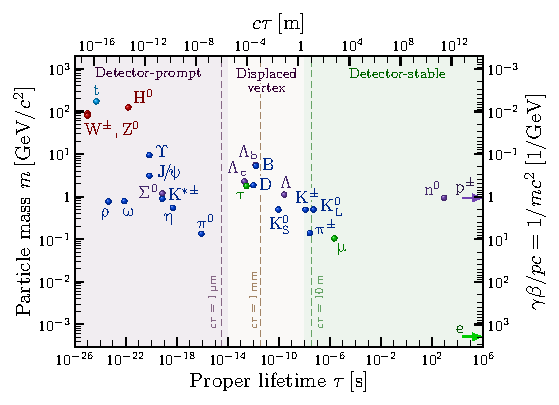
\includegraphics[width=10.5cm]{fig/objects/SM_particles_masses.pdf}
  \vspace{-2mm}
  \caption{
Plot of the mass versus lifetime $\tau$ of many composite and fundamental SM particles.
The decay length is given by $L=\gamma\beta c\tau$, with $\gamma\beta=p/mc$.
Adapted from Ref.~\cite{branching_fractions_fig}.
%Adapted from Ref.~\cite{lifetime_plot}.
  } \label{fig:lifetime}
\end{figure*}
%!TEX root = ../thesis.tex

% FIGURE: PID principles
\begin{figure*}[p!]
  %\vspace{-3mm}
  \centering
  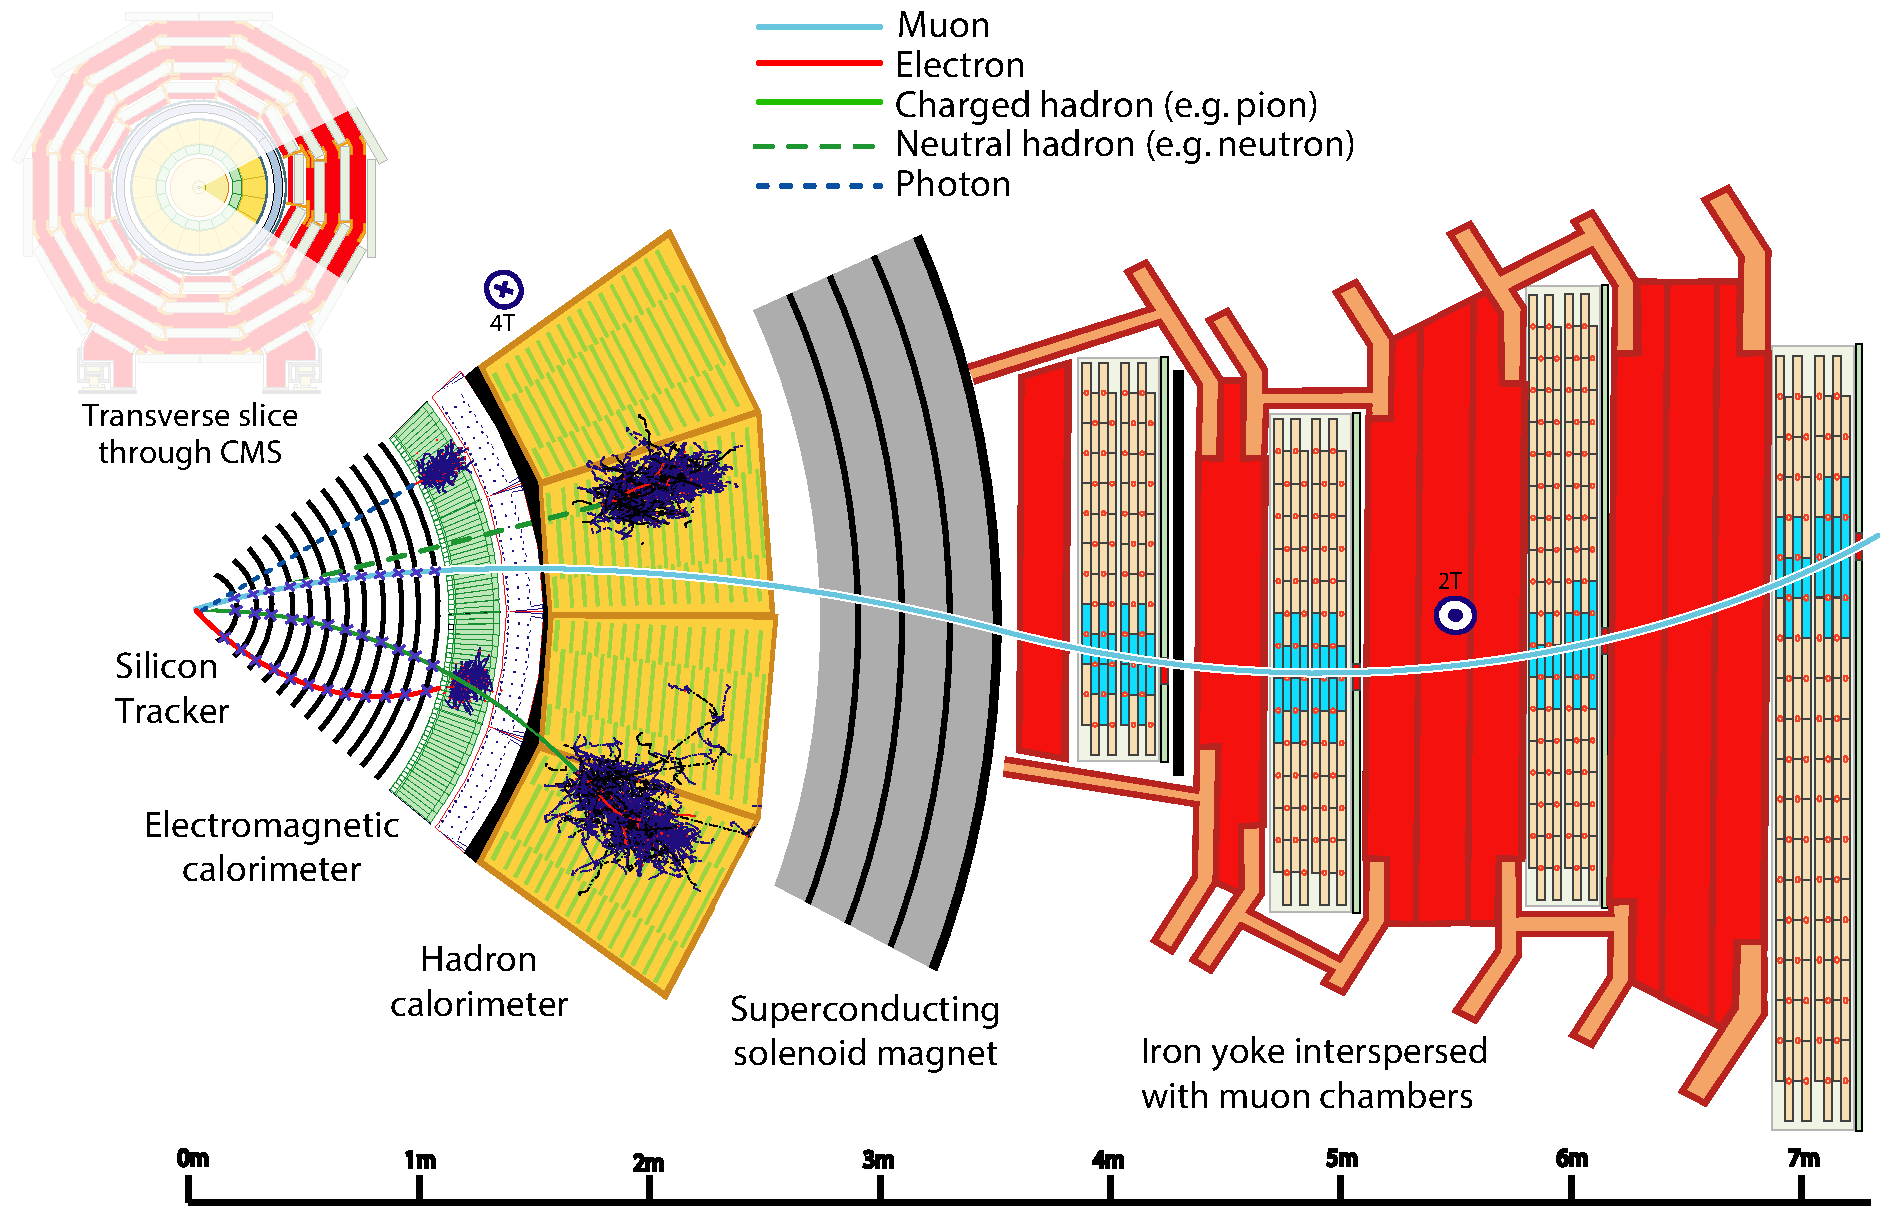
\includegraphics[width=0.92\textwidth]{fig/detector/CMS_detector_PID_edit.pdf}
  \caption{
Particles in the CMS detector.
Adapted from from~\cite{CMS_PID}. % David Barney.
  } \label{fig:PID}
  %\vspace{-3mm}
\end{figure*}


A pp collision event can produce many different types of particles with various masses and lifetimes.
Figure~\ref{fig:lifetime} compares some prominent examples, dividing them in different regions of stability in the context of the CMS experiment.
Electrons, muons, photons, and many hadrons like protons, neutrons, charged pions, and kaons have a lifetime that is long enough to travel through the detector without decaying.
%Other as shown in \Fig{fig:lifetime}.
%like the protons and neutron, but also lighter ones like charged pions $\PGp^\pm$ and kaons.
%The CMS detector detects particles that live long enough to interact with the detector and leave a signal in at least one subdetector.
Each of these particles has a unique set of properties that leave a characteristic signal in one or more of the subdetector, as illustrated in \Fig{fig:PID}.
Electrically charged particles produce ionization in the silicon semiconductors and curve in the magnetic field, whereas neutral particles like neutrons and photons will pass through unbent with little to no interaction. Electrons and photons create electromagnetic showers in the ECAL. Hadrons shower in the HCAL via nuclear interactions, although a shower might already start in the ECAL.
Muons are 207 times heavier than electrons, and are therefore less likely to emit bremsstrahlung and lose energy when moving through matter. This allows high-momentum muons to pass through the whole detector without decaying or being stopped. Muons are characterized by long, single tracks that are picked up by both the tracker and the muon system.
Finally, neutrinos and hypothetical dark matter candidates will escape the detector without leaving any trace. Still, they carry away a large amount of momentum, a fact that can be exploited, as discussed later.

All these signatures are exploited in the reconstruction and identification of objects discussed below. However, these algorithms will never be $100\%$ efficient, nor is there a guarantee that the wrong particle might be identified by an algorithm. Such a particle is referred to as a \emph{fake}. Identification criteria often have several \emph{working points} (WPs) that either have a high efficiency and a high \emph{misidentification rate} (``loose'' WP), or a lower efficiency with a lower misidentification rate (``tight'' WP). The choice of WP is optimized for each analysis.

%, because of \emph{color confinement} in QCD, high-momentum quarks and gluons will fragment into a conical spray of \emph{colorless} hadrons, called a \emph{jet}.
%The detection of quarks and gluons
Collisions also generate high-momentum quarks and gluons, whether from proton debris, hard processes, or from the decay of some particle like the top quark or {\PW} boson.
However, quarks and gluons cannot be isolated as free and stable particles as a consequence of color confinement in QCD. Instead, they hadronizes into a ``jet'' of hadrons as new quark and antiquarks are generated from the strong QCD fields until they form colorless bound states, i.e. hadrons.
CMS reconstructs such jets by grouping particles into cones, as explained in Section~\ref{sec:jets}. 
%(The only exception is the top quark, which is heavier than the $\PW$ boson, and can therefore decay to it before hadronizing.)
% TOP & BOTTOM
%   http://pdg.lbl.gov/2016/tables/rpp2016-tab-mesons-bottom.pdf
%   https://link.springer.com/content/pdf/10.1140/epjc/s10052-018-6459-8.pdf?pdf=button
%   time   = 6.582119e-16/0.3e9 = 2.19e-24
%   length = 1.97327e-7/0.3e9   = 6.58e16 = 0.7 fm
The only exception is the top quark, which decays almost exclusively into a bottom quark and a $\PW$ boson instead of fragmenting into jets like the other quarks~\cite{BR_tt}.
This is because the top's lifetime of $\tau\approx5\times10^{-25}\unit{s}$ is
shorter than the time scale for fragmentation, which is around $10^{-24}\unit{s}$ (or equivalently, a distance scale of about $1\unit{fm}$)~\cite{hadronization_timescale1,hadronization_timescale2}. %or $1\unit{fm}$
%$1/\Lambda_\mathrm{QCD}\sim2\times10^{-24}\unit{s}$. %\mbox{$\sim10^{-8}\unit{ps}$} % 1fm/c
%This means that top quark production will be an important background for analyses with selections of events with leptons plus (b) jet(s), like the one presented in this thesis. Consider for example \mbox{$\ttbar\to\b\b\W^+\W^-$} with the $\W^+\W^-$ pair in a dileptonic final state (with one or two tau leptons), or in the semileptonic final state where one jet is misidentified as a hadronically decaying tau lepton.
%The semileptonic final state of a top quark pair is shown in \Fig{fig:top_pair_decay}.

Bottom quarks produced in high-energy collisions form $\PB$ hadrons that have typical lifetimes of \mbox{$\tau\sim1.5\unit{ps}$}. This is long enough for them to travel a measurable distance of the order of a few millimeters %$\mathcal{O}(3\mm)$ %$\sim p\times100\mum/\text{GeV}$ %450/5.280*30
before decaying and creating a jet known as a \emph{b jet}. This can therefore create a \emph{secondary vertex} that is displaced from its production vertex, which CMS's tracking algorithm can reconstruct.
%This is characteristic of jets originating from bottom quarks, \emph{b jets}.%~\cite{Thea}.
As \Fig{fig:lifetime} shows, $\PGt$ leptons and charmed hadrons are also capable of creating secondary vertices, although each of their decays tend to have a different topology, providing us with some efficiency for distinguishing them with identification algorithms.

Muons and electron candidates can be misidentified jets, or be a real lepton from a hadron decay inside a jet initiated by a quark or a gluon.
%~\cite{HPS2}
Looking at \Fig{fig:lifetime}, we see there are some particles that leave a displaced vertex, and when these are produced in a jet and then decay to a lepton, this lepton may pass standard lepton reconstruction requirements.
%For example, charged pions and kaons can decay mid-flight with $\BR(\PGp^\pm\to\mu^\pm\nu_\mu)\approx100\%$ and $\BR(\PK^\pm\to\ell^\pm X)\approx72\%$, where $\ell=\Pe$, $\PGm$~\cite[p.~33,~40]{PDG_2022}, but in the context of CMS, they are relatively long-lived.
% 71.99 = 1.582e-5+63.56+5.07+3.352+2.55e-5+4.247e-5+1.4e-5+6.2e-3+1.33e-5+9.4e-6+2.66e-4+1.25e-5
Heavy-flavor hadrons are more likely to decay to muons or electrons inside the detector, for example
\mbox{$\PD^\pm\to\ell^\pm X$} ($33.7\%$),
\mbox{$\PD^0\to\ell^\pm X$} ($13.3\%$)~\cite[p.~43,~46]{PDG_2022}.
% 33.67 = 16.07+17.6
% 13.29 = 6.49+6.8
{\PB} hadrons decay to these charmed hadrons, but they themselves also have a significant branching fraction of direct decay to electrons and muons: \mbox{$\BR(\PB\to\ell^\pm X)\approx21\%$}~\cite[p.~54,~61]{PDG_2022}.
%Fig{fig:B_meson_decay} presents the Feynman diagram of a generic $\PB$ hadron decay to a charged lepton and D meson.
It is possible to discriminate against these cases by demanding that the lepton is relatively isolated from other particles with a cone of some $\DR$ size, because jets are typically associated with multiple particles.
%``promptly'', \ie, produced at the PV,


%%%%%%%%%%%%%%%%%%%%%
%   PARTICLE-FLOW   %
%%%%%%%%%%%%%%%%%%%%%
\section{Particle-flow algorithm} \label{sec:PF}
The particle-flow (PF) algorithm~\cite{PF1,PF2017} fully reconstructs the event of a pp collision with an optimized combination of all measurements of the CMS subsystems. %subdetectors.
It first combines signals from different detector components into so-called \emph{PF elements}. These are tracks from the inner tracker, tracks from the muon system, and clusters from calorimeter cells.
These elements are linked together if they are sufficiently close, and are consistent with that expected from electrons, muons, photons, charged hadrons, or neutral hadrons.

Tracks in the inner tracker or muon system are iteratively built from hits, using the \emph{Kalman-filter} (KF) \emph{technique}~\cite{CMS_track_reco_2006,Kalman_filtering}.
%to iteratively built
Calorimeter clusters are built starting from a seed, which is a cell with the largest local energy, after which adjacent cells are iteratively combined into a cluster if their energy exceeds twice the noise level. In the HF, each cell is instead considered a separate cluster.
% 1) tracks Kalman-filter technique, CMS-NOTE-2006-041
% 2) seeds, which are identified as cells with local energy maxima
%    => topological cluster
% 3) An inner track and a calorimeter cluster are linked if the extrapolated track ends up inside the cluster within the uncertainty

Photons are defined as ECAL clusters that are not linked with an extrapolated track, and their energy is obtained from the ECAL measurement.
Charged particle tracks that are not identified as electrons or muons are assumed to be charged hadrons, and their momentum is determined by a combination of the measurements of the calorimeter and tracker, the latter of which is much more precise.
Neutral hadrons are identified from HCAL energy clusters that cannot be linked to any track, or from an energy excess in the ECAL and HCAL that does not fit the expected energy deposit of a charged hadron.
The reconstruction \& identification of electrons and muons will be discussed in more detail below.
The efficiency to correctly identify a track in the barrel with a $\pt$ between $1$ and $100\GeV$ is estimated to be better than $90\%$ for isolated tracks from charged pions and electrons that are isolated, while for muons it is close to $100\%$~\cite{CMS_vertex}.
The \emph{objects} from PF are used to reconstruct objects composed of multiple particles like jets (Section~\ref{sec:jets}) and hadronically decaying $\PGt$ candidates (Chapter~\ref{sec:tauh}), and also to calculate the missing transverse energy (Section~\ref{sec:met}).


%%%%%%%%%%%%%%%%%%%%%%
%   PRIMARY VERTEX   %
%%%%%%%%%%%%%%%%%%%%%%
\section{Primary vertex} \label{sec:PV}
The algorithm locates primary vertices (PVs) of $\Pp\Pp$ collisions by finding tracks that emerge from them in three steps.
It first selects tracks reconstructed by the PF algorithm that extrapolate back to the beam line and pass some quality requirements. 
Then tracks are clustered based on their $z$ coordinate at their point of closest approach to the beam spot using the \emph{deterministic annealing algorithm}~\cite{deterministic_annealing}.
Finally, candidate vertices with at least two associated tracks are fitted using an \emph{adaptive vertex fitter}~\cite{vertex_fitting} to obtain the best vertex parameters.
%and grouping reconstructed tracks that extrapolate back to the same point on the beamline.

The PVs in an event are ordered by the quadratic sum of the $\pt$ of their tracks, $\sum_\text{tracks}\pt^2$.
The one with the largest sum of squared transverse track momenta is assumed to be the vertex of the hard scattering process, while the others are considered to be pileup~\cite{CMS_vertex,PF2017,CMS_vertex_phase2}.
The efficiency to determine the correct vertex with three or more tracks is close to $100\%$~\cite{CMS_vertex}.
The distribution of the number of PVs per beam crossing was shown in \Fig{fig:CMS_pileup}.

% https://cds.cern.ch/record/2683784
The PF algorithm removes the charged hadrons that are assigned to pileup PVs from the collection of objects for physics analysis. This is called \emph{charged-hadron subtraction} (CHS).
As neutral particles from PU cannot be associated with PVs, other correction techniques are needed for jets, lepton isolation, and the identification of hadronically decayed $\PGt$ leptons.

%The electron, muon and tau objects considered in the final selections of this analysis should all fall within a longitudinal distance $d_{z}$ of $0.2\unit{cm}$ and a radial distance $d_{xy}$ of $0.045\unit{cm}$ from the PV, otherwise it is assumed to stem from pileup (PU)



%%%%%%%%%%%%%%%%%
%   ELECTRONS   %
%%%%%%%%%%%%%%%%%
\section{Electrons} \label{sec:electron}

Electrons are reconstructed by associating a track in the inner tracker to clusters of energy deposits in the ECAL.
% tracks
One of the difficulties in reconstructing electrons is that they can emit a significant amount of bremsstrahlung before reaching the ECAL.
This has two effects.
Firstly, it causes significant and sudden changes in their curvature.
As a consequence, the standard tracking algorithm based on the KF may not be able to collect all hits, and may make a poor estimation of the track parameters. That is why candidate tracks are refitted with the \emph{Gaussian sum filter} (GSF)~\cite{GSF}.
%with a small number of hits, or large $\chi^2$
%in addition the Kalman filter by PF
% shower
Secondly, the electron energy is also spread out over several ECAL crystals, mostly along the $\phi$ direction because of the bending of the electron trajectory in the magnetic field.
The ECAL clusters within a certain geometrical window around a seed cluster are therefore recombined into a so-called \emph{supercluster}.
%The PF algorithm recovers some of the energy lost by radiation by matching ECAL clusters that are compatible to the electron track. The energy is then determined by a combination of the track's momentum and the resummation of these associated ECAL clusters.

As estimated from $\PZ\to\Pe\Pe$ decays, the momentum resolution for electrons with a $\pt$ of approximately $45\GeV$ ranges from 1.6 to 5\%.
The resolution is generally better in the barrel region than in the endcaps, and depends on the amount of bremsstrahlung the electron radiates before reaching the ECAL~\cite{CMS_electron_2021,CMS_electron_calibration_2016}.
%as it traverses the material in front of the ECAL.

% ID
Electrons that are produced ``promptly'', \ie, produced at the PV, have several sources of background: photon conversion, hadrons misidentified as electrons, and secondary electrons from hadron decays.
The electron identification is based on discriminating variables that can be grouped into the following three categories:
\begin{enumerate}
  \item variables such as track-cluster matching that compare ECAL and tracker measurements;
  \item ECAL measurements such as shower shapes (electromagnetic showers are typically more narrow than hadronic showers) and energy deposits in the HCAL or endcap preshower; %transversal shower shapes
  \item tracking measurements such as fit parameters (hadrons emit less bremsstrahlung) and separations with respect to charged hadrons.
\end{enumerate}
The electron identification in this analysis is based on a multivariate analysis (MVA): A boosted decision tree (BDT) algorithm~\cite{TMVA} is trained on these variables in bins of $\eta$ and $\pt$.
In addition, electrons must pass the requirement that rejects electrons from photon conversion.
This analysis uses the MVA-based identification with a nominal $90\%$ efficiency WP, based on a training without including isolation variables. %\texttt{MVAFall17V2noIso\_WP90}.
% Ref.
The reconstruction and identification of electrons, as well as high-energy photons, are discussed in more detail in Refs.~\cite{CMS_electron} and~\cite{CMS_electron_2021}.

To discriminate against jets misidentified as leptons, a simple variable to quantify isolation, called the \emph{relative isolation}, is often used.
The most simple version is the sum over the $\pt$ of all PF particles within a cone of some size $\DR$, normalized by the lepton's own momentum, $\pt^\ell$:
\begin{equation} \label{eq:iso_simple}
  \Iell = \frac{1}{\pt^\ell}\sum_\text{particles} \pt.
\end{equation}
This definition is further improved by not considering charged particles that originate from pileup, as well as subtracting the estimated contribution of neutral particles, with the so-called \emph{rho-effective-area method}~\cite{PU_substraction}, quantified by the variable:
%with the so-called \emph{$\Delta\beta$-corrections}:
\begin{equation} \label{eq:iso_ele}
  \Ie \defeq
    \frac{\sum_\text{charged} \PT + \max\left( 0, \sum_\text{neutral} \ET
                                  - \rho A_\text{eff} \right )}{\pt^{\Pe}}. 
\end{equation}
In this expression, $\sum_\text{charged} \pt$ is the scalar $\pt$ sum of the charged hadrons originating from the PV, and located in a cone of size $\DR = 0.3$ centered on the electron direction.
The sum $\sum_\text{neutral} \ET$ represents the same quantity for neutral hadrons and photons with the transverse energy calculated as $\ET=E\sin\theta$.
The neutral contribution from pileup %(photons and neutral hadrons)
is estimated as the event-specific $\rho A_\text{eff}$, where $\rho$ is the average pileup energy density per unit area in the $\phi\eta$ plane, and $A_\text{eff}$ is the effective area in the $\phi\eta$ plane.
For a given $\DR$, the energy density $\rho$ depend roughly linearly on the number of PVs in the event~\cite{CMS_electron}.
In the analysis presented in this analysis, $\Ie < 0.10$ is used as the isolation requirement for the electron.



%%%%%%%%%%%%%
%   MUONS   %
%%%%%%%%%%%%%
\section{Muons} \label{sec:muon}
Muon candidates in CMS are reconstructed as \emph{standalone muons}, \emph{tracker muons}, and/or \emph{global muons}~\cite{CMS_muon_2018}.
%identified by tracks in the central tracker that are consistent with either tracks or several hits in the outer muon detectors.
Standalone muons are tracks that are reconstructed solely from hits in the muon stations.
Conversely, tracker muons are built from tracks reconstructed in the inner tracker that match at least one hit in the DT or CSC segments of the muon system.
Global muons are obtained from standalone muons that match ``inner'' tracks. After finding such a match, a fit to the combined track with the KF is performed in order to improve the muon momentum resolution.
Global muons and tracker muons are merged as a single muon candidate if they share the same inner track.
Owing to the high tracking efficiency, about $99\%$ of muons produced within the geometrical acceptance of the muon system are reconstructed as either a tracker or global muon~\cite{CMS_muon_2018}.
Tracker muons that are not identified as global muons typically originate from remnant of a hadron shower in the HCAL that reaches the inner muon stations (\emph{punch-through}).
The energy and momentum of the muon candidate is determined from the curvature of the track.

A muon identification criterium is defined for three WPs: loose, medium, and tight.
A loose muon is a PF muon that is either a tracker or global muon. These WPs are used to identify prompt muons originating from the PV and ``secondary'' muons from hadron decay, while maintaining a low rate for the misidentification of charged hadrons as muons.
In the analysis for this thesis though, the medium WP is used. A medium muon is a loose muon that passes several quality criteria of the track. %, and matches small energy deposits in the calorimeters.
% eff, fake rate?
%CMS has also a high momentum identification to target muons with $\pt>200$.
% TODO: CHECK IMPROVEMENT STUDY WITH HIGH-PT ID

%Moreover, the data-taking periods B to F suffered some tracking efficiency loss (so-called \emph{HIP effect}). For these data sets, the \emph{medium 2016 ID} for muons has been defined to recover this inefficiency. The data sets G and H, as well as the simulations, use the standard medium-WP identification criteria, \emph{medium ID}, which has about a $10\%$ smaller fake rate for low $\pt$ muons in data than the medium 2016 ID.
%Scale factors are derived to match the efficiency in simulation with the one measured in data, as is explained in Chapter~\ref{sec:corrections}.
%They are measured as an average of the two medium IDs, weighted by corresponding integrated luminosity.

% HTT
%Muons are reconstructed from both the inner tracker and the muon subsystems~\cite{muon}.
%The PF muons are selected from among the reconstructed muon track candidates
%by applying minimal requirements on the track components in the muon system 
%and taking into account matching with small energy deposits in the 
%calorimeters. 
%
%The medium ID is applied to muons in MC simulations. For data events in runs B to F, the ``medium 2016'' ID 
%is used to recover from some tracking inefficiency in that period, and the medium ID is used in runs G and H.
% The medium and medium 2016 ID have about the same efficiency in MC simulations. In runs G and H the medium ID 
%selects approximately 10\% less fake muons in data at low $p_T$, in comparison witn the medium 2016 ID.
%In practice the data/MC scale factors are measured as a weighted combination of the two IDs.

Just like for electrons, the relative isolation of a muon can be defined.
The contribution of neutral particles is taken into account with the so-called \emph{$\Delta\beta$-corrections}:
\begin{equation}\label{eq:iso_mu}
  \Imu \defeq
    \frac{\sum_\text{charged} \pt + \max\left( 0, \sum_\text{neutral} \ET
                                  - \Delta\beta \sum_\text{charged, PU} \pt \right )}{\pt^{\PGm}}.
    %\frac{1}{p_\text{T}^\ell}\left(
    %                \sum_\text{charged} p_\text{T}
    %+ \max\left[ 0, \sum_\text{neutral} p_\text{T} - \Delta\beta \right]
    %\right),
\end{equation}
The muon isolation cone is of angular size $\DR=0.4$.
This expression is similar to \Eq{eq:iso_ele}, but in $\Imu$ the neutral contribution from pileup is estimated from the scalar {\pt} sum of charged hadrons originating from pileup vertices, $\sum_\text{charged, PU} \pt$. This sum is multiplied by a factor of $\Delta\beta = 0.5$, which corresponds approximately to the phenomenological ratio of neutral- to charged-hadron production in the hadronization process of inelastic pp collisions, as estimated from simulation.
%It is approximated with with a neutral-to-charged ratio of $\Delta\beta = 0.5$ in pileup.
%as was done in~\cite{HTT2012,HPS2}.
In the present thesis, $\Imu < 0.15$ is used as the nominal isolation requirement for the muon.



%%%%%%%%%%%%%%%%%%
%%   ISOLATION   %
%%%%%%%%%%%%%%%%%%
%% http://pdg.lbl.gov/2016/tables/rpp2016-tab-mesons-bottom.pdf
%\section{Lepton isolation} \label{sec:iso}
%%\input{tex/AN-16-333-fig-objects_B_meson_decay.tex}
%
%One straightforward way is to quantify the isolation of a lepton by summing over all PF particles within a cone of some size $\DR=\sqrt{\Delta\eta^2+\Delta\phi^2}$, normalized by its own momentum:
%\begin{equation}\label{eq:iso_simple}
%  \Iell = \frac{1}{p_\text{T}^\ell}\sum_\text{particles, \DR} p_\text{T}.
%\end{equation}
%This definition has been further improved by not considering charged particles that originate from pileup, as well as subtracting the contribution of neutral ones with the so-called \emph{$\Delta\beta$-corrections}:
%\begin{equation}\label{eq:iso}
%  \Iell
%    = \frac{1}{p_\text{T}^\ell}\left(
%                    \sum_\text{charged} p_\text{T}
%    + \max\left[ 0, \sum_\text{neutral} p_\text{T} - \Delta\beta \right]
%    \right),
%\end{equation}
%where the neutral particles include photons and neutral hadrons, and $\Delta\beta$ is the neutral component of pileup.
%For electrons this neutral contribution is estimated with a jet area method~\cite{PU_substraction}, while for muons, it is approximated with charged particles from pileup:
%\begin{equation}\label{eq:dbeta}
%  \Delta\beta = 0.5 \sum_\text{charged,PU} p_\text{T},
%\end{equation}
%as was done in~\cite{HTT2012,HPS2}. The factor of $0.5$ is an approximation for the neutral-to-charged ratio in pileup.
%For electrons an isolation cone of $\DR=0.3$ is required. The muon isolation cone is of angular size $\DR=0.4$.
%The electron's isolation cone is smaller since its track is typically less resolved than a muon track, and it leaves wide energy deposits in the ECAL. A smaller isolation cone prevents that other objects that are close, are picked up, and ensures a good efficiency. %ensures a good efficiency of real electrons. % A smaller isolation cone %more narrow, better resolved and %The muon's cone is wider because muon tracks are typically better resolved than electron tracks, while electron




%%%%%%%%%%%%
%   JETS   %
%%%%%%%%%%%%
\section{Jets}\label{sec:jets}

% https://arxiv.org/abs/1706.04965
%These sprays of particles consist of roughly 65% charged hadrons, 25% photons, and 10% neutral hadrons

Jets are most often reconstructed by a sequential clustering algorithm that iteratively groups particles together, based on some measure of distance $d_{ij}$ between two reconstructed objects, and a cut $d_\text{cut}$.
Such an algorithm starts by recombining all particle pairs $(i,j)$ that are closest together in $d_{ij}$, as long as $d_{ij}<d_\text{cut}$. After every step, the recombined pairs are removed from the list and replaced with a ``proto-jet'' that has their summed four-momenta. The algorithm stops when there are no pairs left that pass the cut.

A good jet algorithm must have two criteria.
Firstly, the jet properties must be invariant under the radiation of a soft gluon (\emph{infrared safe}).
Secondly, the reconstruction must be insensitive to the collinear splitting of a particle (\emph{collinear safe}), \ie, if a particle is replaced by two collinear particles who in sum have the same four-momentum.

% anti-kT
There are several infrared and collinear-safe algorithms for jets in CMS.
In this thesis, we use the \emph{anti-$\kt$} (AK) \emph{algorithm}, which utilizes the following metric:
\begin{equation} \label{eq:antikT}
  d_{ij} = \min\left(p_\text{T,i}^{-2},p_\text{T,j}^{-2}\right)\frac{\Delta R^2_{ij}}{\Delta R_y^2},
\end{equation}
where $\Delta R_y$ is a cone size parameter and $\Delta R_y=\sqrt{\Delta y^2+\Delta\phi^2}$ is the distance in $(y,\phi)$-space with the \emph{rapidity}
\begin{equation} \label{eq:rapidity}
  y \defeq \frac{1}{2}\ln\left(\frac{E+p_z}{E-p_z}\right),
\end{equation}
not to be confused with \Eq{eq:dR}, where $y\approx\eta$ if $p\gg m$, leading to \Eq{eq:CMS_eta2}. The $\DR_{ij}$ is the $\DR_y$ distance between particles $i$ and $j$. 
If a cluster $i$ of combined objects satisfies
\begin{equation} \label{eq:antikT_cut}
  d_{ij} > d_{i\text{B}} = p_\text{T,i}^{-2},
\end{equation}
the algorithm defines it to be a jet and removes its PF candidates from consideration in clustering subsequent jets. Here, $d_{iB}$ is called $i$'s distance to the beam~\cite{PF2017,antikT}.
The PF jets are clustered with the standard cone-size parameter \mbox{$\Delta R_y=0.4$}, and are therefore sometimes referred to as ``AK4 jets''.
In CMS, the AK algorithm is implemented in the \FASTJET library~\cite{fastjet1,fastjet2}, and CHS is used to remove charged PF candidates not associated with the PV of the hard interaction.

% JEC
The jet momentum is defined as the vectorial sum of all momenta of the jet constituents.
In order to reconstruct the original quark or gluon accurately and precisely, the energy of jets needs to be calibrated to take into account detector noise and contributions from additional pp interactions within the same or nearby bunch crossings.
%back to particle level, \emph{jet energy corrections} (JEC) are applied.
The CMS Collaboration determines \emph{jet energy corrections} (JECs) in several steps, which are explained in detail in Ref.~\cite{CMS-JME-10-011}.
Additionally, the jet energy and \emph{jet energy resolution} (JER) of jets in simulation are corrected to obtain better agreement between simulation and data.
%~\cite{CMS-JME-10-011}
%An offset correction is applied to jet energies to take into account the contribution from additional pp interactions within the same or nearby bunch crossings~\cite{CMS-JME-10-011}.
%The energy of a jet is calibrated based on simulation and data through correction factors~\cite{CMS-JME-10-011}.
%Due to some mismeasurement of jet energy scale in some runs, jet energy corrections (JEC) need to be applied.
%This is done for data sets with the global tag
%\begin{itemize}
%   \item[] \texttt{80X\_dataRun2\_2016SeptRepro\_v7},
%\end{itemize}
%but not for simulated miniAOD samples with the production global tag
%\begin{itemize}
%  \item[] \texttt{80X\_mcRun2\_asymptotic\_2016\_TrancheIV\_v8}.
%\end{itemize}
%The applied correction labels in data events are \texttt{L1FastJet}, \texttt{L2Relative}, \texttt{L3Absolute} and \texttt{L2L3Residual}.\\
%The simulated jet momentum is on average within 5--10\% of the try momentum, and
%The jet energy resolution typically amounts to 15--20\% at 30\GeV, 10\% at 100\GeV, and 5\% at 1\TeV~\cite{CMS-JME-13-004}.

% JET ID
%Finally, in the present analysis the jets need to pass the loose WP of the PF jet ID discriminator provided.
In the analysis presented in this analysis, two identification requirements are applied in order to distinguish genuine jets from those arising from pileup~\cite{jetPUID}, as well as to remove spurious jet-like features that originate from isolated noise patterns in certain HCAL regions~\cite{jetID_2016}.
The latter is achieved with additional selection criteria on the energy fractions and multiplicity of charged and neutral particles, which corresponds to the ``tight`` jet identification in CMS. It has an almost $100\%$ efficiency for jets with $\pt>30\GeV$ and $\abs{\eta}<0.5$, but degrades down to $97\%$ in the forward region~\cite{jetID_2016}. %quark-initiated 
% OVERLAP REMOVAL
If candidate jets fall within a $\DR<0.5$ from one of the selected $\PGt$ lepton candidates (\ie, an electron, muon, or $\tauh$ object), they are assumed to be the same object, and are removed from the jet collection.
%In this analysis, jets are required to have $\pt>30\GeV$ and $\abs{\eta}<4.7$ for the baseline selections.

%% JETS
%The jets are reconstructed with the infrared and collinear safe $\text{anti-k}_\text{T}$ clustering algorithm with a distance parameter $\DR=0.4$~\cite{jet,antikT}. The jet momentum is determined as the vectorial sum of all particle momenta in this jet, and is found in the simulation to be within 5 to 10\% of the true momentum over the whole \pt spectrum and detector acceptance. Jet energy corrections are derived from the simulation, and are confirmed with in situ measurements with the energy balance of dijet and photon + jet events~\cite{jet_resolution}.



%%%%%%%%%%%%%
%   B TAG   %
%%%%%%%%%%%%%
\section{Bottom quark identification} \label{sec:btagging}
%: TODO: check efficiency

% FIGURE: B TAGGING ILLUSTRATION
%!TEX root = ../thesis.tex

% FIGURE: PID
\begin{figure*}[t!]
  %\vspace{-6mm}
  \centering
  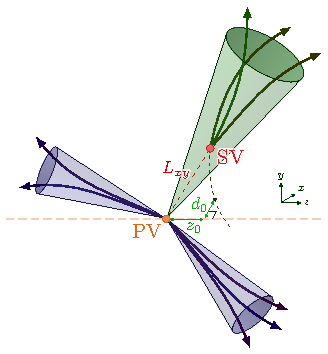
\includegraphics[width=0.33\textwidth]{fig/objects/jet_btag.pdf}
  %\vspace{-2mm}
  \caption{
B-tagging.
  } \label{fig:btagging}
  %\vspace{-8mm}
\end{figure*}


%The relatively long lifetime of B hadrons produced by bottom quarks can be exploited to \emph{b tag} a jet.
As mentioned in Section~\ref{sec:PID}, the relatively long lifetime of $\PB$ hadrons produced by bottom quarks can be exploited to identify bottom-quark intitiated jets.
Besides lifetime, one can exploit the relatively large mass of the {\PB} hadron, and the pattern of fragmentation and decay. This is referred to as \emph{b tagging}.
Most b tagging algorithms use a combination of information about the secondary vertex and track parameters, like the impact parameter (distance of closest approach of the track to the PV), but also exploit information about the jet topology and other properties.
%This analysis uses an improved \emph{Combined Secondary Vertex} (CSVv2) algorithm that inputs these variables into a neural network after making some quality requirements on the track. The output is a value that quantifies the likelihood of the jet to be a b jet. This value can be cut on for different working points. The recommended working points are loose, medium and tight with a fake rate of $10\%$, $1\%$, and $0.1\%$, respectively. This analysis uses a medium WP corresponding to a $0.8484$ requirement on the CSVv2 value~\cite{btag_WP}. The CSV algorithm is described in Ref.~\cite{btag_csv1}, and CSVv2 in Ref.~\cite{btag_csv2}.

The $\LQ\to\btau$ analysis employs the \DeepCSV algorithm~\cite{btag_deepCSV,btag_2018} for b tagging jets. \DeepCSV is a deep neural network (DNN) with four hidden layers that is an extension of the combined secondary vertex (CSV) algorithm~\cite{btag_deepCSV,btag_2018}.
%It exploits observables related to the long lifetime and large mass of {\PQb} hadrons.
The loose and medium working points (WPs) of \DeepCSV are used, which are respectively defined by a 10 and 1\% misidentification rate of jets originating from light quarks or gluons.
The $\eta$ of tagged jets is required to have $\abs{\eta}<2.4$ ($2.5$) in 2016 (2017 and 2018).
Figure~\ref{fig:btag_eff} shows the efficiency and mistag rate for jets in simulated events that pass the selections of the $\mutau$ channel (see Chapter~\ref{sec:selections}) and do not match the selected muon and $\tauh$ candidates within $\DR<0.5$. The efficiency and mistag rates are very similar between the different $\tautau$ decay channels.
The medium WP has a typical efficiency of about 75\%, while the loose WP efficiency can reach up to 90\%, depending on the jet $\pt$ and $\eta$. Nevertheless, the {\PQb} tagging significantly degrades at $\pt \gtrsim 500\GeV$, and more so for the medium than the loose WP.
%The efficiency and mistag rate for jets measured in simulated events passing the {\mutau} or {\ditau} selections are shown in Fig.~\ref{fig:btag_eff}. The efficiency and mistag rates are similar between the channels that are analyzed in this analysis (including the \etau and \emu channels).

% FIGURE: B TAG EFFICIENCIES
\input{tex/corrections-fig-btag.tex}



%%%%%%%%%%%
%   MET   %
%%%%%%%%%%%
% https://twiki.cern.ch/twiki/bin/view/CMSPublic/WorkBookMetAnalysis#7_7_6_MET_Corrections
\section{Missing transverse energy}\label{sec:met}
%!TEX root = ../thesis.tex

% FIGURE: MET
\begin{figure*}[t]
  %\vspace{-6mm}
  \centering
  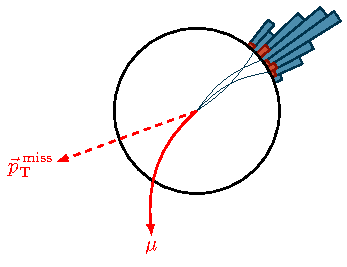
\includegraphics[width=0.39\textwidth]{fig/objects/transverse_plane.pdf}
  %\vspace{-2mm}
  \caption{
Illustration of missing transverse energy (MET) with a muon track (red), and energy deposits in the calorimeters.
  } \label{fig:MET}
  %\vspace{-2mm}
\end{figure*}

As mentioned in Section~\ref{sec:pp_collisions}, the longitudinal boost of the hard scattering is unknown, but the total transverse momentum is assumed to be exactly zero and conserved. This is useful to infer invisible particles that have carried away a significant amount of momentum, like neutrinos or hypothetical dark matter particles.
After the PF algorithm has reconstructed all particles in the event and removed charged particles not coming from the PV, it vectorially sums the remaining objects to determine the total transverse momentum that is missing:
\begin{equation} \label{eq:MET}
  \ptvecmiss = - \sum_{\text{i}}\myvec{p}_\text{T}^{\,i}.
\end{equation}
This vector, or its length, is often referred to as the \emph{missing transverse momentum}, or \emph{missing transverse energy} (MET).
%then is simply the vector $E_\text{T}^\text{miss} = \left|\myvec{p}_\text{T}^\text{\,miss}\right|$.
The accuracy of the MET relies on a good calibration of all PF objects.
Therefore, the calibration of the jet energy scale has to be propagated correctly.
Several other corrections are applied, for example, in case the computed MET is very large, the PF algorithm checks for cosmic muons, badly reconstructed muon tracks, and fake muons~\cite{PF2017}.
More details can be found in Refs.~\cite{CMS-PAS-JME-16-004} and~\cite{CMS-PAS-JME-17-001}. 
%In this analysis, Type-1 corrections that take into account the JEC are applied.
%There are also Type-0 and Type-2 corrections, which are discussed in Ref.~\cite{MET_types}.
%The missing transverse energy is defined as the negative vectorial sum of the transverse momenta of all PF candidates. Type-1 corrections are applied to the transverse missing energy, as well as recoil corrections, which are described in the next section.



%%%%%%%%%%%%%%
%   D_ZETA   %
%%%%%%%%%%%%%%
%%%\section{$D_\zeta$ observable} \label{sec:dzeta}
%%%To suppress backgrounds from top quark pair and \W + jets production, the variable called $D_\zeta$ is defined. This observable was introduced in a $\H\to\tt$ analysis at CDF~\cite{pzeta}. In this analysis it is only considered in the \emu channel.
%%%The $D_\zeta$ variable is constructed as follows: An axis $\zeta$ is defined as the bisector of the visible transverse momenta of the two tau decay products (e.g. the electron and muon in the $\tt\to\emu$ channel), $\myvec{p}_\text{T,1}^\text{\,vis}$ and $\myvec{p}_{T,2}^\text{\,vis}$. The sum of $\myvec{p}_\text{T,1}^\text{\,vis}$ and $\myvec{p}_\text{T,2}^{\text{\,vis}}$ is projected on the $\zeta$-axis with and without the missing transverse momentum $\myvec{p}_{T}^\text{mis}$ with some factor for optimization:
%%%\begin{align} \label{eq:pzeta}
%%%  \myvec{p}_{\zeta}^\text{\,vis} &\equiv
%%%               (\myvec{p}_\text{T,1}^\text{\,vis} + \myvec{p}_\text{T,2}^\text{\,vis})
%%%               \frac{\myvec{\zeta}}{|\vec{\zeta}|}, \\
%%%  \myvec{p}_{\zeta} &\equiv
%%%               (\vec{p}_\text{T,1}^\text{\,vis} + \myvec{p}_\text{T,2}^\text{\,vis} + \myvec{p}_\text{T}^\text{mis})
%%%               \frac{\myvec{\zeta}}{|\vec{\zeta}|}.
%%%\end{align}
%%%The construction of $\myvec{p}_\zeta$ and $\myvec{p}^\text{\,vis}_\zeta$ is illustrated in Fig.~\ref{fig:pzeta}.
%%%$D_\zeta$ is now defined as the magnitude of the difference of these projections:
%%%\begin{equation} \label{eq:dzeta}
%%%  D_{\zeta} \equiv p_{\zeta} - 1.85 p_{\zeta}^\text{vis}.
%%%\end{equation}
%%%This variable quantifies the compatibility of events with the topology wherein the direction of missing neutrinos from $\tau$ decays are aligned with the direction of the visible $\tau$ decay products. In the \emu channel the quantities $\myvec{p}_{T,1}^\text{\,vis}$ and $\myvec{p}_{T,2}^\text{\,vis}$ correspond to the transverse momenta of the electron and muon.
%%%
%%%\input{tex/AN-16-333-fig-objects_pzeta.tex}



